
%\vspace{-0.05in}
\section{Chain Wielding Strategies for Markov-chain Monte Carlo Estimators in Inclusive Variational Inference}
\vspace{-0.05in}
\subsection{Overview of Prevoius Estimation Strategies}\label{section:jsa_msc}
%
\vspace{-0.05in}

\paragraph{Overview}
Recently,~\citeauthor{NEURIPS2020_b2070693} and~\citeauthor{pmlr-v124-ou20a} proposed two similar but independent methods for performing inclusive variational inference.
Both methods estimate the score gradient by operating a Markov-chain in parallel with the VI optimization sequence.
Also, they both use MCMC kernels that can effectively used the variational approximation \(q_{\vlambda_t}(\vz)\).
Because of this, compared to previous VI approaches~\citep{pmlr-v97-ruiz19a, pmlr-v70-hoffman17a} that use expensive MCMC kernels such as Hamiltonian Monte Carlo, both methods are computationally efficient. 

\vspace{-0.05in}
\paragraph{Markovian Score Climbing and the Single State Estimator}
In Markovian score climbing (MSC), \citep{NEURIPS2020_b2070693} estimate the score gradient by performing an MCMC iteration and update the parameters such that
\vspace{-0.05in}
\begin{align}
  &\vz_t \sim K\left(\vz_{t-1}, \cdot \right) &g_{\text{single-CIS}}(\vlambda) = s\,(\vz_t; \vlambda)
\end{align}
where \(K\left(\vz_{t-1}, \cdot\right)\) is a MCMC kernel leaving \(p\,(\vz\mid\vx)\) invariant and \(g_{\text{single}}\left(\vlambda\right)\) denotes the score estimator.
For \(K\left(\vz_{t-1}, \cdot\right)\), they propose a new type of kernel inspired by particle MCMC~\cite{andrieu_particle_2010}, the conditional importance sampling (CIS) kernel.
Since the estimator uses \textit{a single state} created by the CIS kernel, we call it the single state estimator with the CIS kernel (single-CIS).
The CIS kernel internally uses \(N\) samples from the \(q_{\vlambda}(\vz)\).
Thus, when compared to MCMC kernels that only use a single sample from \(q_{\vlambda}(\vz)\), it is \(N\) times more expensive, but hopefully, statistically superior.
Unfortunately, we will show that this is not the case.

\vspace{-0.05in}
\paragraph{Joint Stochastic Approximation and the Sequential State Estimator}
On the other hand, at each SGD iteration \(t\),~\citep{pmlr-v124-ou20a} perform \(N\) sequential Markov-chain transitions and use the average of the intermediate states for estimation.
That is, for the index \(i \in \{1, \ldots, N\}\),
\vspace{-0.05in}
\begin{align}
  &\vz_{T+i} \sim K^i\left(\vz_{T}, \cdot \right) &g_{\text{seq.-IMH}}(\vlambda) = \frac{1}{N} \sum_{i=1}^N s\,(\vz_{T+i}; \vlambda)
\end{align}
where \(\vz_T\) is the last Markov-chain state of the previous SGD iteration.
For the MCMC kernel, they use the classic independent Metropolis-Hastings (IMH,~\citealt[Algorithm 25]{robert_monte_2004}~\citealt{hastings_monte_1970}) algorithm, which uses only a single sample from \(q_{\vlambda}(\vz)\).
Therefore, the cost of \(N\) state transitions with IMH is similar to the cost of a single transition with CIS.
Since the estimator uses sequential states, we call it the sequential state esimator with the IMH kernel (seq.-IMH)

\vspace{-0.05in}
\paragraph{Additional  Notes on JSA}
Before preoceeding, we acknowledge that the setup of~\citet{pmlr-v124-ou20a} is slightly different than what we described.
Their MCMC kernel leave \(p\left(\vz_j\mid\vx_j \right)\) invariant for a single datapoint \(\vx_j\), which is only possible when the datapoints are independently, identically distributed (\textit{iid}) under the probabilistic model.
We interpret their method more generally and assume that we only have a kernel that can leave \(p\left(\vz\mid\vx \right)\) invariant.

\subsection{Overview of Markov-Chain Monte Carlo Score Estimation Strategies}\label{section:overview}

\begin{figure*}
  \vspace{-0.4in}
    \centering
    \begin{subfigure}[b]{0.25\textwidth}
        \centering
        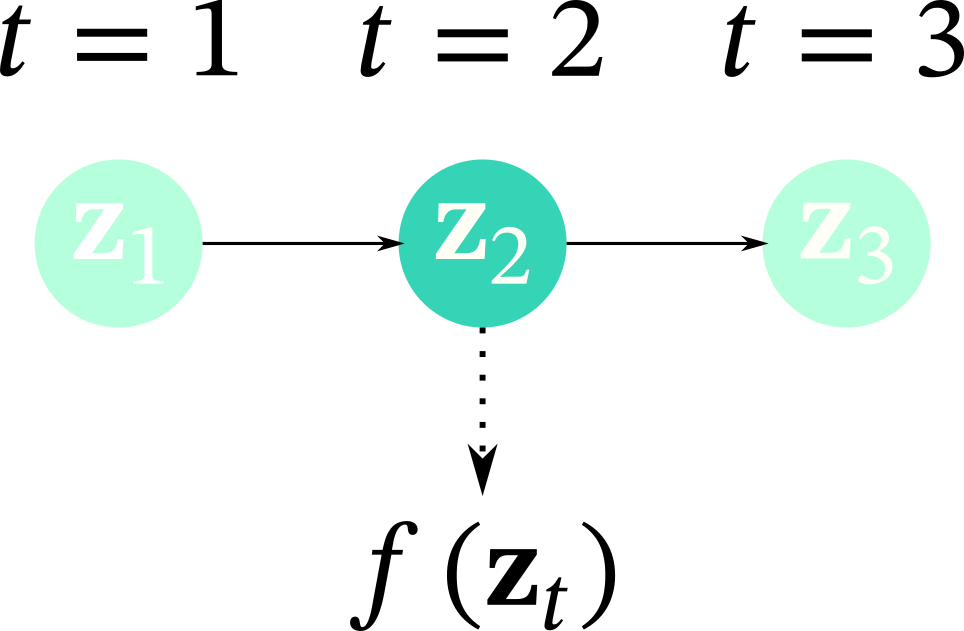
\includegraphics[scale=0.25]{figures/diagram_1.png}
        \caption{Single state estimator}\label{fig:single}
    \end{subfigure}
    \begin{subfigure}[b]{0.35\textwidth}
        \centering
        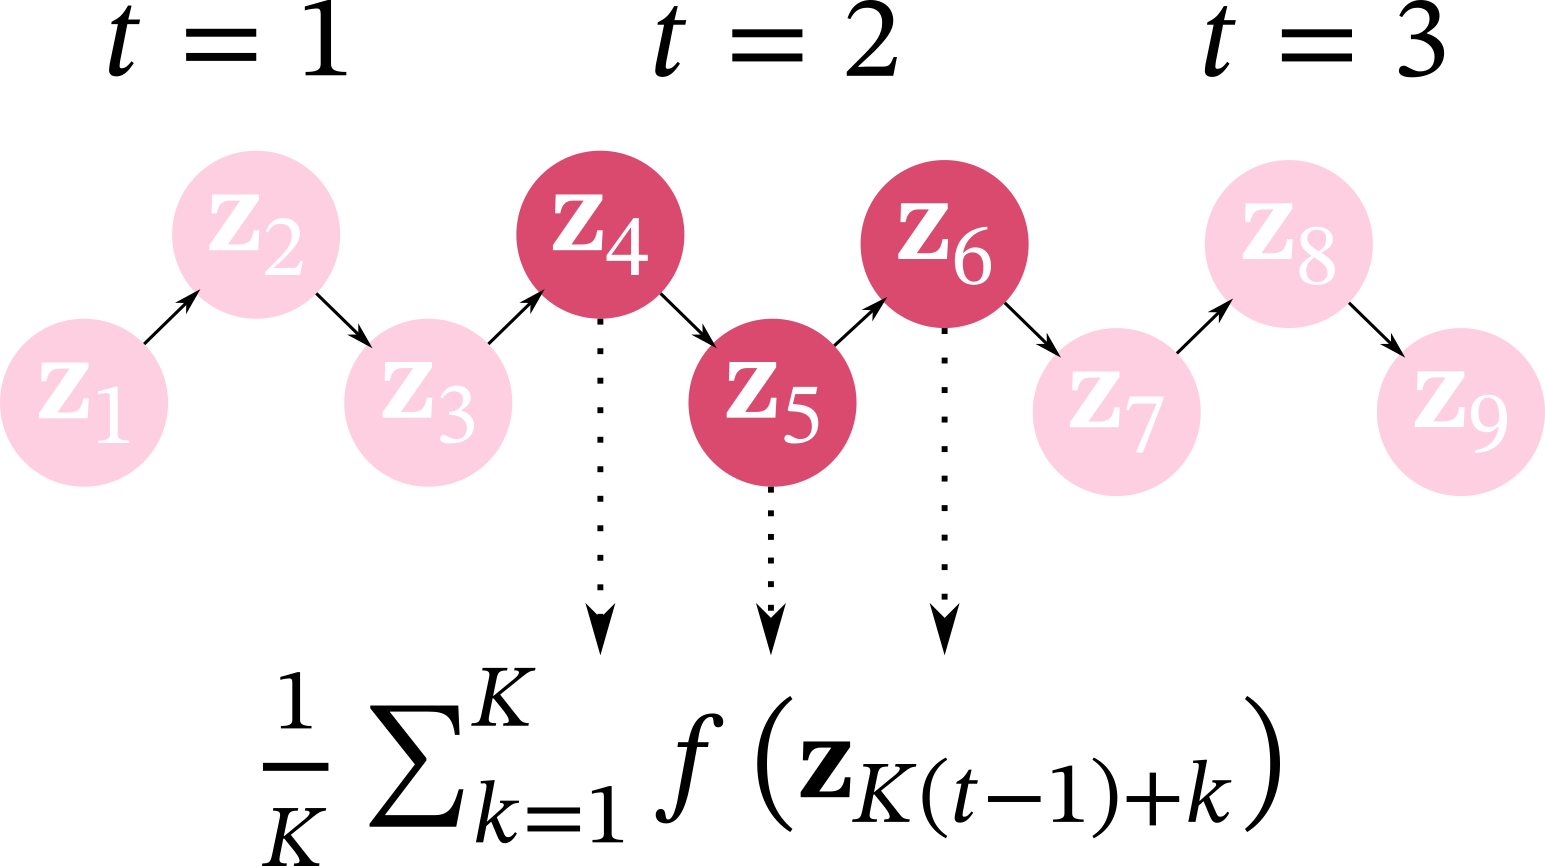
\includegraphics[scale=0.25]{figures/diagram_2.png}
        \caption{Sequential state estimator}\label{fig:seq}
    \end{subfigure}
    \begin{subfigure}[b]{0.3\textwidth}
        \centering
        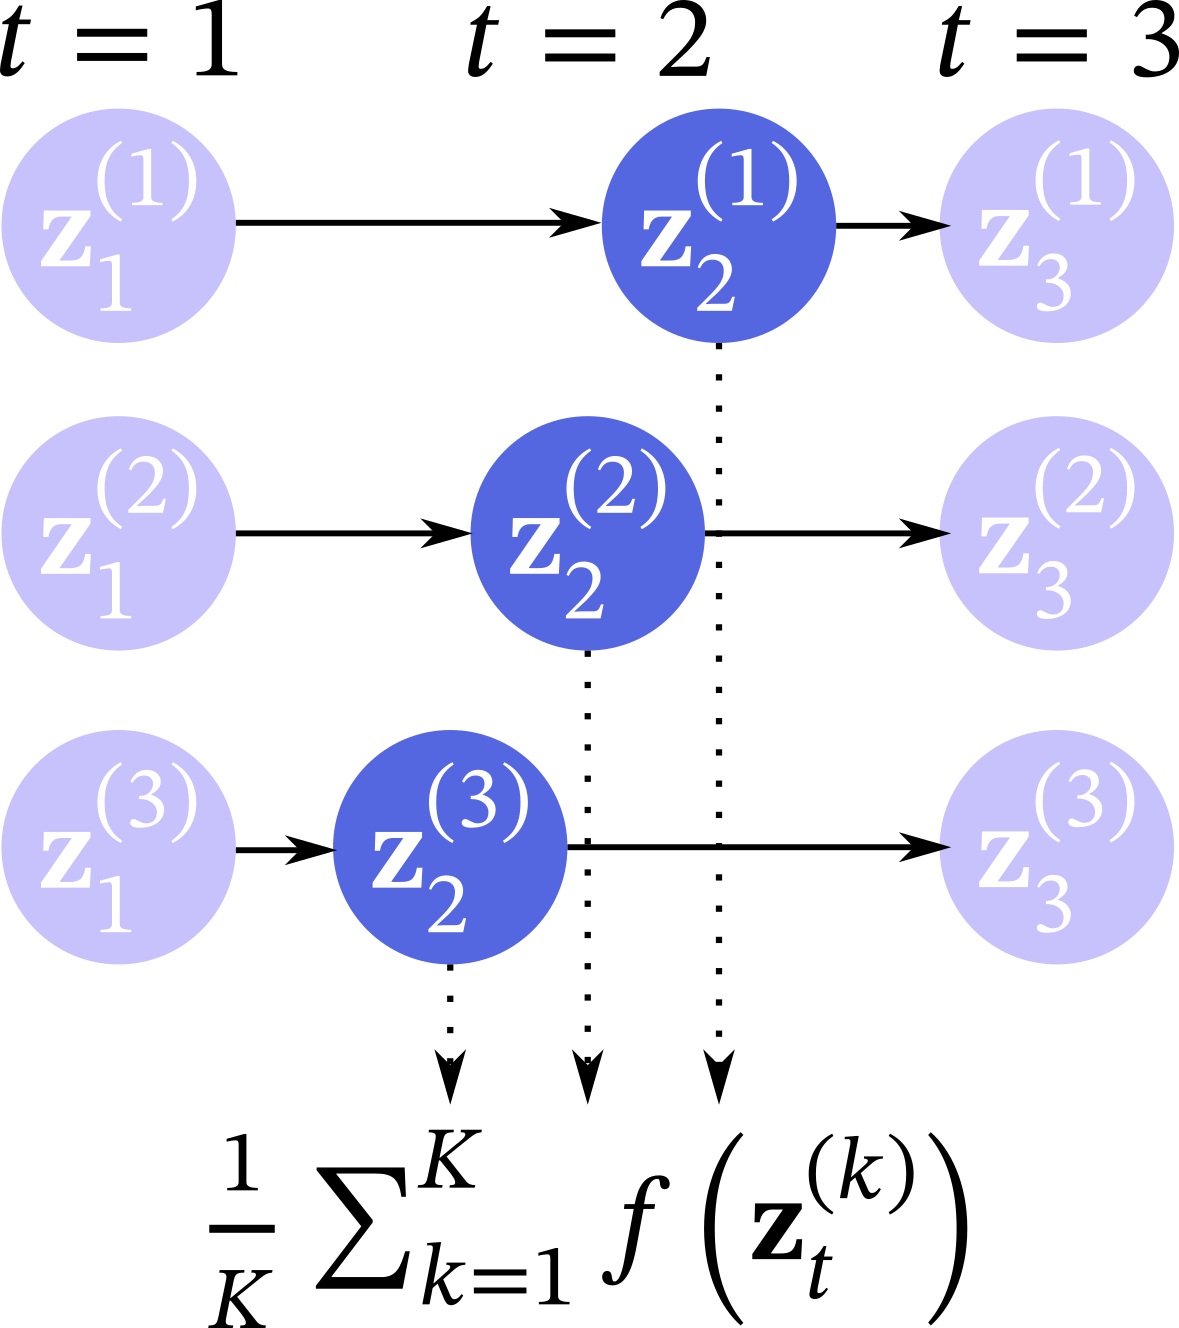
\includegraphics[scale=0.25]{figures/diagram_3.png}
        \caption{Parallel state estimator}\label{fig:par}
    \end{subfigure}
    \caption{Visualization of different ways of combining MCMC with stochastic approximation variational inference.
    The index \(t\) denotes the stochastic approximation iteration.
    The dark circles denote the MCMC samples used for estimating the score gradient at \(t=2\).
    }\label{fig:overview}
\end{figure*}

\vspace{-0.05in}
\paragraph{Single State and Sequential State Estimators}
The two different MCMC estimators used in MSC and JSA represent two different ways of using a fixed computational budget.
The former uses a computationally expensive, but hopefully statistically superior, MCMC kernel with less samples, while the latter uses a cheaper MCMC kernel with more samples.
Illustrations of the two schemes are shown in~\cref{fig:single,fig:seq}.
Detailed pseudocodes of the considered schemes are provided in the \textit{supplementary material}.

\vspace{-0.05in}
\paragraph{Parallel State Estimator}
In this work, we will add a new scheme into the mix: the parallel state estimator.
Similarly with the sequential state estimator, we use the cheaper IMH kernel, but instead of applying the MCMC kernel \(N\) times to a single chain, we apply the MCMC kernel a single time to \(N\) \textit{parallel Markov-chains}.
That is, for each Markov-chain \(i \in \{1, \ldots, N\}\),
%
\vspace{-0.05in}
\begin{align}
  &\vz_{t}^{(i)} \sim K\big(\vz_{t-1}^{(i)}, \cdot \big) &g_{\text{par.-IMH}}(\vlambda) = \frac{1}{N} \sum_{i=1}^N s\,(\vz_{t}^{(i)}; \vlambda)
\end{align}
%
where \(\vz_{t-1}^{(i)}\) is the state of the \(i\)th chain at the previous SGD step.
Computationally speaking, we are still applying \(K\big(\vz_{t-1}^{(i)}\big)\) \(N\) times in total, so the cost is similar to the sequential state estimator.
However, the Markov-chain are \(N\) times shorter, which, in a traditional MCMC view, might seem to result in worse statistical performance.
An illustration of the parallel state estimator is shown in~\cref{fig:par}

%

% Second version of table, with booktabs.
%\begin{table}
%\centering
\caption{Computational Costs of MCSA Schemes}\label{table:cost}
\setlength{\tabcolsep}{0.5pt}
  \begin{threeparttable}
\begin{tabular}{lccccc}\toprule
& \multicolumn{3}{c}{\footnotesize Kernel Application} & \multicolumn{2}{c}{\footnotesize Gradient Estimation} \\
\cmidrule(lr){2-4}\cmidrule(lr){5-6}
  & {\footnotesize\(p\left( \vz, \vx \right)\)}
  & {\footnotesize\(q\left(\vz; \vlambda\right)\)}
  & {\footnotesize\(q\left(\vz; \vlambda\right)\)}
  & {\footnotesize\(p\left( \vz, \vx \right)\)}
  & {\footnotesize\( q\left(\vz; \vlambda\right)\)}
  \\
  & {\footnotesize\# Eval.  }
  & {\footnotesize\# Eval.  }
  & {\footnotesize\# Samples}
  & {\footnotesize\# Grad.  }
  & {\footnotesize\# Grad.  }
%
\\\midrule
%
{\footnotesize
ELBO
}
& \(0\)
& \(0\)
& \(N\)
& \(N\)
& \(N\)
\\\arrayrulecolor{black!30}\midrule
%
{\footnotesize
MSC
}
& \(N-1\)
& \(N\)
& \(N-1\)
& \(0\)
& \(1\)\tnote{1}\;\;{\footnotesize or}\;\(N\)\tnote{2}
\\
%
{\footnotesize
JSA
}
& \(N\)
& \(N+1\)
& \(N\)
& \(0\)
& \(N\)
\\
%
{\footnotesize
\textit{pMCSA}
}
& \(N\)
& \(2 \, N\)
& \(N\)
& \(0\)
& \(N\)
\\\bottomrule
\end{tabular}
  \begin{tablenotes}
    \item[*]{\footnotesize We assume that the parameters are cached as much as possible}.
    \item[1]{\footnotesize Vanilla CIS kernel}.
    \item[2]{\footnotesize Rao-Blackwellized CIS kernel}.
  \end{tablenotes}
  \end{threeparttable}
%\end{table}

%
\paragraph{Computational Cost}
The three scheme using the CIS kernel and the IMH kernel can have different computational cost depending on the parameter \(N\).
The computational costs of each scemes are organized in~\cref{table:cost}.
In the CIS kernel, \(N\) controls the number of internal proposals sampled from \(q_{\vlambda}(\vz)\).
In the sequential and parallel state estimators, the IMH kernel only uses a single sample from \(q_{\vlambda}(\vz)\), but applies the kernel \(N\) times.
When estimating the score, the single state estimator computes \(\nabla_{\vlambda} q_{\vlambda}(\vz)\) only once, while for the sequential and parallel state estimators compute it \(N\) times.
However,~\cite{NEURIPS2020_b2070693} also discuss a Rao-Blackwellized version of the CIS kernel, which also computes the gradient \(N\) times.

\subsection{Theoretical Analysis}

\textcolor{red}{
  \paragraph{Boundedness Assumption}
Since we derive our bounds on the bias from the total-variation distance, our results assume that the score function is bounded.
That is, \(\norm{\nabla_{\vlambda} \log q_{\vlambda}(\vz)} < L\) for any \(\vlambda\).
This boundedness assumption is reasonable since theoretical guarentees of SGD often assume Lipschitz-continuity of the gradients, from which boundedness follow as a consequence.
}


\begin{theoremEnd}{propossition}\label{thm:bias_seq}
  Assuming \(w^* = \sup_{\vz} \nicefrac{p\left(\vz\mid\vx\right)}{q_{\vlambda_{t}}\left(\vz\right)} < \infty\; \text{for} \; \forall \vlambda \) and the score function is bounded such that \(\left|\,s(\vz; \vlambda)\,\right| \leq \frac{L}{2}\), the bias of the sequential state estimator with an IMH kernel at iteration \(t\) is bounded as
  {\small
  \[
    \mathrm{Bias}\left[ g_{\mathrm{seq.,\, t}} \right] \leq \frac{L}{N} \, (w^* - 1)
  \]
  }
\end{theoremEnd}
%
\begin{proofEnd}
  We employ a similar proof strategy with the works of~\citet[Theorem 4]{jiang_mcmc_2021}.

  Let us first denote the empirical distribution of the Markov-chain states at iteration \(t\) as
  \begin{align}
    \eta_{\mathrm{seq.},\, t}(\vz) = \frac{1}{N} \sum_{i=1}^N K^{i}(\vz_T, \vz),
  \end{align}
  where \(\vz_{T}\) is the last state of the Markov-chain at the previous SGD iteration.
  Consequently, the estimator can be described as
  \begin{align}
      g_{\mathrm{seq}, t}(\vlambda) = \int s\left(\vz; \vlambda\right) \, \eta_{\mathrm{seq.},\, t}(\vz) \, d\vz.
  \end{align}
  Now,
  \begin{align}
    \DTV{ \eta_{seq.,\, t}(\cdot) }{p\left(\cdot\mid\vx\right)}
    &= \DTV{\frac{1}{N} \sum_{i=1}^N K^{i}(\vz_T, \cdot)}{p\left(\cdot\mid\vx\right)} \\
    &\leq \frac{1}{N} \sum_{i=1}^N  \DTV{K^{i}(\vz_T, \cdot)}{p\left(\cdot\mid\vx\right)} &\text{ (Triangle inequality)}
  \end{align}
 For an IMH kernel with \(w^* < \infty\), the geometric ergodicity of the IMH kernel \citep[Theorem 2.1]{10.2307/2242610} gives the bound
 \begin{align}
   \DTV{K^t(\vz_{0}, \cdot)}{p(\cdot\mid\vx)} \leq {\left(1 - \frac{1}{w^*}\right)}^t.
 \end{align}
 For the SGD step \(t\), \(\vlambda_{t}\) is fixed, temporarily enabling ergodicity to hold.
 Therefore, 
  \begin{align}
    \DTV{ \eta_{\mathrm{seq.},\, t}(\cdot) }{p\left(\cdot\mid\vx\right)}
    &\leq \frac{1}{N} \sum_{i=1}^N {\left( 1 - \frac{1}{w^*} \right)}^i \\
    &=    \frac{1}{N} \sum_{i=1}^N C^i \\
    &=    \frac{1}{N} \left(\frac{ C \left(1 - C^{N}\right)}{1 - C}\right) \\
    &=    \frac{C}{N} \frac{ \left(1 - C^{N}\right) }{1 - C} \\
    &\leq \frac{1}{N} \frac{ C }{1 - C} \\
    &=    \frac{1}{N} \frac{ 1 - \nicefrac{1}{w^*} }{ \nicefrac{1}{w^*} } \\
    &=    \frac{1}{N} \left( w^* - 1 \right)
  \end{align}

  Finally, by the definition of the total-variation distance, 
 \begin{align}
   \mathrm{bias}\left[ g_{\mathrm{seq., t}} \right]
   &\leq \DTV{\eta_{seq.,\, t}(\cdot)}{p(\cdot\mid\vx)} \\
   &\leq \sup_{h : \mathcal{Z} \rightarrow \left[ \text{-}\nicefrac{L}{2}, \nicefrac{L}{2} \right]} \left|\, \Esub{\eta_{\mathrm{seq.},\, t}(\cdot)}{h} - \Esub{p(\cdot\mid\vx)}{h} \,\right| \\
   &= L \, \DTV{ \eta_{\mathrm{seq.},\, t}(\cdot) }{p\left(\cdot\mid\vx\right)}  \\
   &\leq \frac{L}{N} \left( w^* - 1 \right).
 \end{align}
\end{proofEnd}

%%% Local Variables:
%%% TeX-master: "master"
%%% End:

%
For the sequential mode estimator, the bias depends on both \(t\) and \(N\).
Thus, the bias decreases as the number iteration \(t\) and the number of samples \(N\) increase.
However, the following proposition suggests that the \(w^*\) will be exponentially large when the KL divergence is large.
%
\begin{proposition}
  \(w^* = \sup_{\vz} \nicefrac{p\left(\vz\mid\vx\right)}{q_{\vlambda}\left(\vz\right)} \) is bounded below expoentially by the KL divergence such that
  \(
  \exp\left(\DKL{p\left(\cdot\mid\vx\right)}{ q_{\vlambda}\left(\cdot\right) }\right) \leq w^*.
  \)
  \begin{proof}
    \(
    \DKL{p\left(\cdot\mid\vx\right)}{ q_{\vlambda}\left(\cdot\right) }
    = \int p\left(\vz\mid\vx\right) \log \frac{p\left(\vz\mid\vx\right)}{q_{\vlambda}\left(\vz\right)}\,d\vz
    \leq \int p\left(\vz\mid\vx\right) \log M \, d\vz = \log w^*
    \)
  \end{proof}
\end{proposition}
%
Therefore, in the initial iterations of VI when the KL divergence has yet been minimized, the constant \(C\) will be close to 1.
On the other hand, when \(C\) is small, the bias will be small regardless of \(N\) and \(t\).
Thus, increasing \(N\) wouldn't result in significant bias reduction.


\begin{theoremEnd}{theorem}
  Assuming \(w^* = \sup_{\vz} \nicefrac{p\left(\vz\mid\vx\right)}{q_{\vlambda_{\tau}}\left(\vz\right)} < \infty \; \text{for}\;\forall \vlambda \) and that the score function is bounded as \(\left|\, s\left(\vz; \vlambda\right) \,\right| \leq \frac{L}{2}\), the bias of the parallel mode estimator with an IMH kernel at iteration \(t\) is bounded as
  {\small
\[
    \mathrm{Bias}\left[ g_{\mathrm{par.,\, t}} \right] \leq L\,C^t.
\]
  }
  where \(C = 1 - \nicefrac{1}{w^*}\).
\end{theoremEnd}
\begin{proofEnd}
  We denote the empirical distribution of the Markov-chain states at iteration \(t\) as
  \begin{align}
    \eta_{\mathrm{par.},\, t}(\vz) = \frac{1}{N} \sum_{i=1}^N K^{t}\left(\vz_0^{(i)}, \vz\right).
  \end{align}
  and consequently,
  \begin{align}
      g_{\mathrm{par.}, t}(\vlambda) = \int s\left(\vz; \vlambda\right) \, \eta_{\mathrm{par.},\, t}(\vz) \, d\vz.
  \end{align}
  Similarly with~\cref{thm:bias_seq}, 
  \begin{align}
    \DTV{ \eta_{\mathrm{par.},\, t}(\vz) }{p\left(\cdot\mid\vx\right)}
    &= \DTV{\frac{1}{N} \sum_{i=1}^N K^{t}\left(\vz_0^{(i)}, \vz\right)}{p\left(\cdot\mid\vx\right)} \\
    &\leq \frac{1}{N} \sum_{i=1}^N  \DTV{K^t(\vz_0^{(i)}, \cdot)}{p\left(\cdot\mid\vx\right)} &\text{(Triangle inequality)} \\
    &=    \DTV{K^t(\vz_0, \cdot)}{p\left(\cdot\mid\vx\right)} &\text{(Independence)} \\
    &\leq \prod_{\tau=1}^t {\left(1 - \frac{1}{w^*(\vlambda_{\tau})}\right)} \\
    &\leq \prod_{\tau=1}^t {\left(1 - \frac{1}{w^*}\right)} \\
    &\leq C^t
  \end{align}
  where \(w^*(\vlambda_{\tau}) = \sup_{\vz} \nicefrac{p\left(\vz\mid\vx\right)}{q_{\vlambda_{\tau}}\left(\vz\right)} \) and \(C = 1 - \nicefrac{1}{w^*}\).
  And, finally the bias is given as
 \begin{align}
   \mathrm{bias}\left[ g_{\mathrm{par., t}} \right]
   &\leq L \DTV{\eta_{\mathrm{par.},\, t}(\cdot)}{p(\cdot\mid\vx)} \\
   &\leq L \sup_{h : \mathcal{Z} \rightarrow \left[ \text{-}\nicefrac{L}{2}, \nicefrac{L}{2} \right]} \left|\, \Esub{\eta_{\mathrm{par.},\, t}(\cdot)}{h} - \Esub{p(\cdot\mid\vx)}{h} \,\right| \\
   &= L\, \DTV{ \eta_{\mathrm{par.},\, t}(\cdot) }{p\left(\cdot\mid\vx\right)}  \\
   &\leq L \, C^t.
 \end{align}
\end{proofEnd}

%%% Local Variables:
%%% TeX-master: "master"
%%% End:


\textit{Detailed derivation of \textbf{\cref{eq:var_seq}}}

First, remember that the estimator is defined as
  \begin{align*}
    \vg_{\text{seq.}}\left(\vlambda\right) = \frac{1}{N} \sum_{i=1}^N \vs\left(\vlambda; \vz_{T+i}\right),
  \end{align*}
where \( \vz_{T+i} \sim K_{\vlambda_{t-1}}^i\left( \vz_{T}, \cdot \right) \) and \(\vz_T\) is the last Markov-chain state at the previous SGD iteration \(t-1\).
Then, the variance is given as

\begin{align*}
  \V{g_{\text{seq.}}}
  &= \V{ \Esub{K\left(\vz_{T}, \vz\right)}{ \frac{1}{N} \sum_{i=1}^N \vs\left(\vlambda; \vz_{T+i}\right)  \,\Bigg\vert\, \vz_T } }
  + \E{ \Vsub{K\left(\vz_{T}, \vz\right)}{ \frac{1}{N} \sum_{i=1}^N \vs\left(\vlambda; \vz_{T+i}\right) \,\Bigg\vert\,  \vz_T } } &\text{(Total Variance)}  \\
  &= \frac{1}{N^2} \sum_{i=1}^N \Vsub{K\left(\vz_{T}, \vz\right)}{ \E{  \vs\left(\vlambda; \vz_{T+i}\right) \mid \vz_T } }  \\
  &\qquad + \E{ \frac{1}{N^2}  \sum_{i=1}^N  \Vsub{K\left(\vz_{T}, \vz\right)}{ \vs\left(\vlambda; \vz_{T+i}\right)  \mid  \vz_T } 
+ \frac{2}{N^2}  \sum_{i < j}^N \Cov{ s\left(\vlambda; \vz_{T+i}\right), \vs\left(\vlambda; \vz_{T+j}\right) \mid  \vz_T }
  }  \\
  &= \frac{1}{N^2} \sum_{i=1}^N \Vsub{K\left(\vz_{T}, \vz\right)}{ \E{  \vs\left(\vlambda; \vz_{T+i}\right) \mid \vz_T } }  \\
   &\qquad+ \frac{1}{N^2} \sum_{i=1}^N   \Esub{K\left(\vz_{T}, \vz\right)}{ \V{ \vs\left(\vlambda; \vz_{T+i}\right)  \mid  \vz_T } } 
   + \frac{2}{N^2}  \sum_{i < j}^N \E{ \Cov{ \vs\left(\vlambda; \vz_{T+i}\right), \vs\left(\vlambda; \vz_{T+j}\right) \mid  \vz_T }
  },
\intertext{\text{where by assuming stationarity such that \(\vz_{T} \sim p\left(\vz \mid \vx \right)\),}}
  &= \frac{1}{N^2} \sum_{i=1}^N \Vsub{p\left(\vz_T \mid \vx \right)}{ \E{  \vs\left(\vlambda; \vz_{T+i}\right) \mid \vz_T } } 
   \qquad+ \frac{1}{N^2} \sum_{i=1}^N   \Esub{p\left(\vz_T \mid \vx \right)}{ \V{ \vs\left(\vlambda; \vz_{T+i}\right)  \mid  \vz_T } } \\
 &\qquad+ \frac{2}{N^2}  \sum_{i < j}^N \E{ \Cov{ \vs\left(\vlambda; \vz_{T+i}\right), \vs\left(\vlambda; \vz_{T+j}\right) \mid  \vz_T }
  } \\
  &= \frac{1}{N^2} \sum_{i=1}^N \Vsub{p\left(\vz \mid \vx \right)}{ \vs\left(\vlambda; \vz\right) } 
 + \frac{2}{N^2}  \sum_{i < j}^N \E{ \Cov{ \vs\left(\vlambda; \vz_{T+i}\right), \vs\left(\vlambda; \vz_{T+j}\right) \mid  \vz_T }
  }&\text{(Total Variance)} \\
  &= \frac{1}{N} \Vsub{p\left(\vz \mid \vx \right)}{ \vs\left(\vlambda; \vz\right) } 
 + \frac{2}{N^2}  \sum_{i < j}^N \E{ \Cov{ \vs\left(\vlambda; \vz_{T+i}\right), \vs\left(\vlambda; \vz_{T+j}\right) \mid  \vz_T }
  } \\
  &= \frac{\sigma^2}{N}
 + \frac{2}{N^2}  \sum_{i < j}^N \E{ \Cov{ \vs\left(\vlambda; \vz_{T+i}\right), \vs\left(\vlambda; \vz_{T+j}\right) \mid  \vz_T }
  }
\end{align*}

%%% Local Variables:
%%% TeX-master: "master"
%%% End:


\subsection{Interpreting Conditional Importance Sampling as Independent Metropolis-Hastings}\label{section:cis_imh}
Many popular MCMC kernels are based on the Metropolis-Hastings test where a random proposal \(\vz^*\) is either accepted into the Markov-chain (\(\vz_{t} = \vz^*\)) or rejected (\(\vz_t = \vz_{t-1}\)).
Among these, independent Metropolis-Hastings (IMH) kernels generate proposals independently of \(\vz_{t-1}\) such as \(\vz^* \sim q\,(\vz)\) instead of \(\vz^* \sim q\,(\vz\mid\vz_{t-1})\).% for \textit{state-dependent}.
%This constrasts with other kernels that generate  proposals such as .
We show that the CIS kernel proposed by~\citet{NEURIPS2020_b2070693} turns out to be a type of IMH kernel that uses Barker's acceptance ratio~\citep{barker_monte_1965} for the Metropolis-Hastings test.
This interpretation enables the analysis of the \textit{rejection rate} of the CIS kernel.

\vspace{-0.1in}
\paragraph{Conditional Importance Sampling}
A pseudocode of the CIS kernel is shown in~\cref{alg:cis}.
The original algorithmic description of CIS is to
\begin{enumerate*}[label=(\roman*)]
  \item obtain \(N\) samples from \(q_{\vlambda}(\vz)\),
  \item compute the importance weight including the previous Markov-chain state \(\vz_{t-1}\), and 
  \item resample \(\vz_{t-1}\) from the multinomial distribution of \(N+1\) proposals.
\end{enumerate*}
%
While particle MCMC~\citep{andrieu_particle_2010} originally inspired the CIS kernel, it is possible to find connections in multiple-try MCMC methods~\citep{martino_review_2018}.
In particular, the CIS kernel is identical to the previously proposed \textit{ensemble MCMC sampler}~\citep{austad_parallel_2007, neal_mcmc_2011a} with independent proposals, which is an instance of multiple-try MCMC~\citep[Table 12]{martino_review_2018}.

\vspace{-0.1in}
\paragraph{CIS as a Metropolis-Hastings Kernel}
Now we show that the CIS kernel is an accept-reject type kernel with Barker's acceptance ratio.
First, by defining \(\vz_t = \vz_{t-1}\) as ``reject'' and \(\vz_t \neq \vz_{t-1}\) as ``accept'', the CIS kernel can be understood as an accept-reject type kernel.
By denoting the \(N\) parallel proposals as an \textit{ensemble state} \(\vz^{(1:N)} = (\vz^{(1)}, \ldots, \vz^{(N)})\)~\citep{neal_mcmc_2011a}, the CIS kernel conditional estimate can be written as
%
{%\small
  \begin{align}
    \Esub{K(\vz_{t-1}, \vz_t)}{f(\vz_t)\mid\vz_{t-1}}  = 
    \Esub{q_{\vlambda}}{
      \alpha\,(\vz_{t-1}, \vz^{(1:N)}) \,
      \frac{
        \sum^{N}_{i=1} w\,(\vz^{(i)})\,f(\vz^{(i)})
      }
           {
             \sum^{N}_{i=1} w\,(\vz^{(i)})
           }
    }
    + r\,(\vz_{t-1}) \, f(\vz_{t-1})\label{eq:cis_kernel}
  \end{align}
}
where \(q_{\vlambda}(\vz^{(1:N)}) = \prod^N_{i=1} q_{\vlambda}(\vz^{(i)}) \),
the acceptance ratio
\(
  \alpha(\vz_{t-1}, \vz^{(1:N)})
  = \nicefrac{\sum^{N}_{i=1} w\,(\vz^{(i)})}{\sum^{N}_{i=0} w\,(\vz^{(i)})}
\)
is the probability of accepting the ensemble state \(\vz^{(1:N)}\), and
\begin{align}
  r\,(\vz_{t-1}) = \Esub{q_{\vlambda}(\vz^{(1:N)})}{
    r\,(\vz_{t-1} \mid \vz^{(1:N)})
  }
  = \Esub{q_{\vlambda}(\vz^{(1:N)})}{
    \left(1 - \alpha\,(\vz_{t-1}, \vz^{(1:N)})\right)
  }
\end{align}
is the probability of staying on \(\vz_{t-1}\) by rejecting \textit{any} ensemble state, \(r\,(\vz_{t-1}\mid \vz^{(1:N)})\) is the rejection rate given \(\vz^{(1:N)}\).
The expression of \(\alpha\,(\vz_{t-1}, \vz^{(1:N)})\) is known as Barker's acceptance ratio~\citep{barker_monte_1965}, which is a special case of the original Metropolis ratio~\citep{metropolis_equation_1953}.
(A detailed derivation is in the \textit{supplementary material}.)

%% Now, the transition kernel can be denoted as
%% \begin{align}
%%   K(\vz_{t-1}, \vz) = \int K(\vz^{(1:N)}, \vz) \, \big( 1 - r\,(\vz_{t-1}\mid\vz^{(1:N)}) \big) \, q_{\vlambda}( \vz^{(1:N)} ) \, d\vz^{(1:N)}
%%   + r\,(\vz_{t-1}) \,\delta_{\vz_{t-1}}(\vz)
%% \end{align}

\subsection{Bias-Variance Tradeoff of Conditional Importance Sampling}\label{section:bias_variance}
\paragraph{Variance of Conditional Importance Sampling}
The IMH (or accept-reject) view in~\cref{section:cis_imh} now enables us to discuss the rejection rate of the CIS kernel.
As discussed in~\cref{section:msc_mcmc}, MSC obtains gradients using the conditional estimates of MCMC.
The variance of the conditional estimate is closely related to the rejection rate such as
\begin{align}
  \Vsub{K(\vz_{t-1},\cdot)}{f \mid \vz_{t-1}} 
  &=\Vsub{q_{\vlambda}}{ \E{ f \mid \vz_{t-1},\,\vz^{(1:N)} } } + \underbrace{\Esub{q_{\vlambda}}{ \V{ f \mid \vz_{t-1},\,\vz^{(1:N)} } }}_{\text{Rao-Blackwellization gain}} \label{eq:total_variance} \\
  &\geq \Vsub{q_{\vlambda}}{ \E{ f \mid \vz_{t-1},\,\vz^{(1:N)} } } \label{eq:rao_blackwell}\\
  &= \Vsub{q_{\vlambda}}{ \big(1 - r\,(\vz_{t-1}\mid\vz^{(1:N)})\big)\, f_{\mathrm{IS}}
    + r\,(\vz_{t-1}\mid\vz^{(1:N)})\,f(\vz_{t-1}) \;\middle\vert\; \vz_{t-1} } \label{eq:exact_variance} \\
  &\text{where}\;\; f_{\mathrm{IS}} = {\sum_{i=1}^N w\,(\vz^{(i)}) f(\vz^{(i)})\,/\,\sum_{i=1}^N w\,(\vz^{(i)})}. \nonumber 
\end{align}
%
The bound in~\eqref{eq:rao_blackwell} becomes exact if we use Rao-Blackwellization (that is, if we use the SNIS estimator \(\sum^{N}_{i=1} \widetilde{w}^{(i)}\,f\,(\vz^{(i)})\) instead of the resampled \(\vz_t\)) as mentioned by~\citet{NEURIPS2020_b2070693}.
The expansion in~\eqref{eq:total_variance} follows from the law of total variance where the right-hand term is the variance reduction we gain from using Rao-Blackwellization~\citep{bernton_locally_2015}, and the equality in~\eqref{eq:exact_variance} follows from~\eqref{eq:cis_kernel}.

\vspace{-0.1in}
\paragraph{Low rejection rate means high conditional variance.}
Because of the dependence of \(r\,(\vz_{t-1}\mid\vz^{(1:N)})\) on \(\vz^{(1:N)}\), it is in general difficult to interpret the result of~\eqref{eq:exact_variance}.
Nonetheless, when \(w\,(\vz_{t-1}) \gg w\,(\vz^{(i)})\), \(r(\vz\mid\vz^{(1:N)})\) is close to 1 almost independently of \(q_{\vlambda}(\vz)\).
The intuition is that if the \textit{rejection weight} \(w\,(\vz_{t-1})\) is large, most proposals will be rejected regardless of their values.
By translating this intuition into an approximation, we obtain the following result.
%

\begin{theoremEnd}{proposition}\label{thm:approx_var}
  Assuming \(w\,(\vz_{t-1})\) is large enough to make \(r\,(\vz\mid\vz^{(1:N)})\) independent of \(\vz^{(1:N)}\), the variance can be approximated by
  \begin{align}
    \Vsub{q_{\vlambda}}{ \E{ f \mid \vz_{t-1}, \vz^{(1:N)} } } \approx {\big(1 - r\,(\vz_{t-1})\big)}^2\,\Vsub{q_{\vlambda}}{ f_{\text{IS}} \,\middle\vert\, \vz_{t-1} }.
  \end{align}
\end{theoremEnd}
\begin{proofEnd}
  We evaluate the variance by approximating the rejection probability as an independent constant.
  First,
  \begin{align}
    &\Vsub{q_{\vlambda}}{ \E{ f \mid \vz_{t-1}, \vz^{(1:N)} } }. \\
    \intertext{
      Applying~\eqref{eq:cis_kernel_inter},
    }
    &= \Vsub{q_{\vlambda}}{ \big(1 - r\,(\vz_{t-1}\mid\vz^{(1:N)})\big)\, f_{\mathrm{IS}}
      + r\,(\vz_{t-1}\mid\vz^{(1:N)})\,f(\vz_{t-1}) \;\middle\vert\; \vz_{t-1}} \\
    &\approx \Vsub{q_{\vlambda}}{ \big(1 - r\,(\vz_{t-1})\big)\, f_{\mathrm{IS}}
      + r\,(\vz_{t-1})\,f(\vz_{t-1}) \;\middle\vert\; \vz_{t-1}} \\
    &= \Vsub{q_{\vlambda}}{ \big(1 - r\,(\vz_{t-1})\big)\, f_{\mathrm{IS}} \;\middle\vert\; \vz_{t-1} } \label{eq:approx_var_constant} \\
    &= {\big(1 - r\,(\vz_{t-1})\big)}^2 \, \Vsub{q_{\vlambda}}{ f_{\mathrm{IS}} \;\middle\vert\; \vz_{t-1} }. \label{eq:approx_var_linear} 
  \end{align}
  The equality of~\eqref{eq:approx_var_constant} follows from the fact that \(r\,(\vz_{t-1})\,f(\vz_{t-1})\) is a constant.
\end{proofEnd}

%%% Local Variables:
%%% TeX-master: "master"
%%% End:

%
The statement of~\cref{thm:approx_var} is intuitive; if we reject all the states, there is no conditional variance.
However, this obvious fact becomes more interesting combined with the followings.

\vspace{-0.1in}
\paragraph{CIS has a high rejection rate until MSC converges.}
The following bound provides a condition for the rejection rate of a CIS kernel to be high.
%

\begin{theoremEnd}[]{proposition}\label{thm:cis_bound}
  The rejection rate \(r\,(\vz_{t-1})\) of a CIS sampler with \(N\) proposals is bounded below such that
  \[
  %r(\vz_{t-1}) \geq \frac{1}{1 + N\frac{q_{\vlambda}(\vz_{t-1})}{p(\vz_{t-1}\mid\vx)}}.
  r\,(\vz_{t-1}) \geq \frac{w\,(\vz_{t-1})}{w\,(\vz_{t-1}) + N\,Z}
  \]
  where \(Z=\Esub{q_{\vlambda}(\vz)}{\nicefrac{p(\vz,\vx)}{q_{\vlambda}(\vz)}} = \int p\,(\vz,\vx)\,d\vz\) is the normalizing constant.
\end{theoremEnd}
\begin{proofEnd}
  The rejection rate \(r(\vz_{t-1})\) is given as
  \begin{align}
    r(\vz_{t-1})
    &= \Esub{q_{\vlambda}}{ \frac{w(\vz_{t-1})}{ \sum^{N}_{k=1} w(\vz^{(k)}) + w(\vz_{t-1})} } \\
    &= \Esub{q_{\vlambda}}{ {\left( \frac{\sum^{N}_{k=1} w(\vz^{(k)}) }{ w(\vz_{t-1}) } + 1 \right)}^{-1} }.  \\
\intertext{At this point, we apply Jensen's inequality subject to the convex function \(f(x) = \nicefrac{1}{(1 + x)}\),}
    &\geq \frac{1}{1 + \Esub{q_{\vlambda}}{ \frac{\sum^{N}_{k=1} w(\vz^{(k)})}{w(\vz_{t-1})} } } \\
    &=    \frac{1}{1 + \frac{1}{w(\vz_{t-1})} \Esub{q_{\vlambda}}{ \sum^{N}_{k=1} w(\vz^{(k)}) } }. \\
\intertext{From the independence of the \(N\) proposals, we obtain}
    &=    \frac{1}{1 + \frac{1}{w(\vz_{t-1})} N \Esub{q_{\vlambda}}{ w(\vz) } } \\
    &=    \frac{1}{1 + \frac{1}{w(\vz_{t-1})}\,N\,Z } \\
    &=    \frac{w(\vz_{t-1})}{w(\vz_{t-1}) + N\,Z}.
  \end{align}
\end{proofEnd}

%%% Local Variables:
%%% TeX-master: "master"
%%% End:

%
When \(w\,(\vz_{t-1})\) is large, the lower bound of \(r(\vz_{t-1})\) becomes close to one.
In this case, according to~\cref{thm:approx_var}, the conditional variance becomes minimal.

In the context of VI, the following shows that \(r\,(\vz_{t-1})\) is huge when the KL divergence is large.
%

\begin{theoremEnd}[]{theorem}\label{thm:cis_bound_kl}
  Assuming \(\sup_{\vz} \nicefrac{p(\vz\mid\vx)}{q_{\vlambda}(\vz)} = M < \infty\), the average rejection rate \(r = \int r(\vz_{t-1}) \, p(\vz_{t-1}\mid\vx) \, d\vz_{t-1} \) of a CIS kernel with \(N\) proposals is bounded below such that
  \[
  r \geq 1 \big/ 
    \left(1 + \frac{N}{
      \exp\big(\DKL{p}{q_{\vlambda}}\big)
    }
    \right) - \delta,
  \]
  where \(
  0 \leq \delta \leq \frac{M}{\exp^2\,\big( \DKL{p}{q_{\vlambda}}\big) }
  \)
  is the sharpness of the bound, and \(Z = \int p\,(\vz,\vx) \, d\vz\).
\end{theoremEnd}
\begin{proofEnd}
  We first show a simple Lemma that relates the rejection weight \(w\,(\vz_{t-1})\) with the KL divergence.
  \begin{framedlemma}\label{thm:rej_kl_bound}
    The average unnormalized weight of the rejection states is bounded below by the KL divergence such as
    \[
    Z\,\exp\big(\DKL{p}{q_{\vlambda}}\big) \leq \Esub{p(\vz_{t-1}\mid\vx)}{w\,(\vz_{t-1})}.
    \]
  \begin{proof}
    By the definition of the inclusive KL divergence,
    \begin{align}
      \DKL{p}{q_{\vlambda}} = \int p\,(\vz\mid\vx) \log \frac{p\,(\vz\mid\vx)}{q_{\vlambda}(\vz)} \, d\vz
      &\leq \log \Esub{p(\vz\mid\vx)}{\frac{p\,(\vz\mid\vx)}{q_{\vlambda}(\vz)}} \\
      &= \log \Esub{p(\vz\mid\vx)}{ \frac{w\,(\vz)}{Z} } \label{eq:weight_bound_kl}
    \end{align}
    where the right-hand side follows from Jensen's inequality.
    By a simple change of notation, we relate~\eqref{eq:weight_bound_kl} with the rejection states \(\vz_{t-1}\) such as
    \begin{align}
      \DKL{p}{q_{\vlambda}} &\leq \log \Esub{p(\vz_{t-1}\mid\vx)}{\frac{w\,(\vz_{t-1})}{Z}}.
    \end{align}
    Then,
    \begin{align}
      \exp\big(\DKL{p}{q_{\vlambda}}\big) &\leq \Esub{p(\vz_{t-1}\mid\vx)}{
        \frac{w\,(\vz_{t-1})}{Z}} \\
      Z \exp\big(\DKL{p}{q_{\vlambda}}\big) &\leq \Esub{p(\vz_{t-1}\mid\vx)}{w\,(\vz_{t-1})}.
    \end{align}
  \end{proof}
  \end{framedlemma}
  Now, from the result of~\cref{thm:cis_bound},
  \begin{equation}
    \Esub{p(\vz_{t-1}\mid\vx)}{ r(\vz_{t-1}) } \geq \Esub{p(\vz_{t-1}\mid\vx)}{ \frac{w(\vz_{t-1})}{w(\vz_{t-1}) + N\,Z}} =
    \Esub{p(\vz_{t-1}\mid\vx)}{ \varphi\left( w(\vz_{t-1}) \right)  },\label{eq:mean_bound}
  \end{equation}
  where \(\varphi(x) = \nicefrac{x}{(x + N\,Z)}\).
  The lower bound has the following relationship
  \begin{equation}
    \varphi\left(\,
    \Esub{p(\vz_{t-1}\mid\vx)}{ w(\vz_{t-1}) }
    \,\right)
    \geq
    \Esub{p(\vz_{t-1}\mid\vx)}{ \varphi\,\left( w\,(\vz_{t-1}) \right)  }
  \end{equation}
  by the concavity of \(\varphi\) and Jensen's inequality.
  From this, we denote the \textit{Jensen gap}
  \begin{equation}
    \delta = 
    \varphi\left(\,
    \Esub{p(\vz_{t-1}\mid\vx)}{ w(\vz_{t-1}) }
    \,\right)
    -
    \Esub{p(\vz_{t-1}\mid\vx)}{ \varphi\,\big( w(\vz_{t-1}) \big)  }\label{eq:jensen_gap}
  \end{equation}
  where \(\delta \geq 0\).
  Then, by applying~\eqref{eq:jensen_gap} to~\eqref{eq:mean_bound},
  \begin{align}
    \Esub{p(\vz_{t-1}\mid\vx)}{ r(\vz_{t-1}) }
    &\geq \Esub{p(\vz_{t-1}\mid\vx)}{ \varphi\,\big( w\,(\vz_{t-1}) \big)  } \\
    &= \varphi\left(\,
    \Esub{p(\vz_{t-1}\mid\vx)}{ w(\vz_{t-1}) }
    \,\right) - \delta, \\
\intertext{and by the monotonicity of \(\varphi\) and~\cref{thm:rej_kl_bound},}
    &\geq \varphi\left(\,
    Z\,\exp\big(\DKL{p}{q_{\vlambda}}\big)
    \,\right) - \delta \\
    &=
    \frac{
      Z\,\exp\big(\DKL{p}{q_{\vlambda}}\big)
    }{
      Z\,\exp\big(\DKL{p}{q_{\vlambda}}\big) + N\,Z
    } - \delta \\
    &= \frac{
      \exp\big(\DKL{p}{q_{\vlambda}}\big)
    }{
      \exp\big(\DKL{p}{q_{\vlambda}}\big) + N
    } - \delta \\
    &= \frac{1}{
       1 + \frac{N}{
         \exp\big(\DKL{p}{q_{\vlambda}}\big) 
      }
    } - \delta.
  \end{align}
  We lastly discuss the Jensen gap \(\delta\), which directly gives the sharpness of our lower bound.
  \citet[Theorem 1]{liao_sharpening_2019} showed that, for a random variable \(X \in (a, b), -\infty \leq a < b \leq \infty\) and a \textit{convex} function \(\widetilde{\varphi}\,(x)\), the Jensen gap is bounded such that
  \begin{align}
    \E{\widetilde{\varphi}\,(x)} - \widetilde{\varphi}\,(\E{x})
    \leq
    \sup_{x \in (a,b)} h\,(x; \mu) \, \sigma^2
    \quad \text{where}\quad h\,(x; \nu) = \frac{\widetilde{\varphi}\,(x) - \widetilde{\varphi}\,(\nu)}{{(x - \nu)}^2} - \frac{ \widetilde{\varphi}\,\prime(\nu) }{ x - \nu },\label{eq:jensen_gap_bound}
  \end{align}
\(\mu\) and \(\sigma^2\) are the mean and variance of \(X\).
Also, \citet[Lemma 1]{liao_sharpening_2019} show that, if \(\varphi\prime\,(x)\) is concave,  \(\sup_{x \in (a,b)} h\,(x; \mu) = \lim_{x \rightarrow a} h\,(x; \mu) \). 

In our case, the domain is \((a,b) = (0, \infty)\) since \(w\,(\vz_{t-1}) \geq 0\).
We then define our convex function \(\widetilde{\varphi}\,(x) = - \varphi\,(x)\).
Since \(\varphi\,\prime(x) = \nicefrac{N\,Z}{{(x + N\,Z)}^2}\) is convex, \(\widetilde{\varphi}\,\prime(x)\) is concave. Then, 
\begin{align}
  \lim_{x \rightarrow 0} h\,(x; \mu)
  &=
  \lim_{x \rightarrow 0} \; \frac{1}{{(x - \mu)}^2} \left( \widetilde{\varphi}\,(x) - \widetilde{\varphi}\,(\mu) \right)
  - \frac{1}{ x - \mu }  \widetilde{\varphi}\,\prime(\mu)  \\
  &=
  \lim_{x \rightarrow 0} \frac{1}{{(x - \mu)}^2}
  \left(
  - \frac{x}{x + N\,Z} + \frac{\mu}{\mu + N\,Z}
  \right)
  -
  \frac{1}{x - \mu}
  \left(
  - \frac{N\,Z}{ {(\mu + N\,Z)}^2 }
  \right) \\
  &= \frac{1}{\mu^2} \left( \frac{\mu}{\mu + N\,Z} \right)
  - \frac{1}{\mu} \left( \frac{N\,Z}{{(\mu + N\,Z)}^2} \right) \\
  &= \frac{1}{ \mu \, (\mu + N\,Z) }
  - \frac{N\,Z}{ \mu \, {(\mu + N\,Z)}^2} \\
  &< \frac{1}{\mu^2}
\end{align}
Notice that in the context of the original problem, \(\mu = \Esub{p(\vz_{t-1}\mid\vx)}{ w\,(\vz_{t-1}) }\).
We obtain the relationship with our original problem as
\begin{align}
  \delta
  = \varphi\,(\E{x}) - \E{\varphi\,(x)}
  = \E{-\varphi\,(x)} - \varphi\,(-\E{x})
  = \E{\widetilde{\varphi}\,(x)} - \widetilde{\varphi}\,(\E{x}).
\end{align}

We finally discuss the variance term \(\sigma^2\) present in~\eqref{eq:jensen_gap_bound}.
Since we assume \(\sup \nicefrac{p\,(\vz\mid\vx)}{q_{\vlambda}(\vz)} = M < \infty \), \( 0 < \frac{p\,(\vz\mid\vx)}{q_{\vlambda}(\vz)} < M \) for all \(\vz \in \mathcal{Z}\).
Then, since the variance is defined as
\begin{align}
    \sigma^2 &= \E{w^2\,(\vz)} - {\E{w\,(\vz)}}^2 \\
             &= \E{ {\left( \frac{Z\,p\,(\vz\mid\vx)}{q_{\vlambda}(\vz) } \right)}^2 } - {\E{\frac{Z\,p\,(\vz\mid\vx)}{q_{\vlambda}(\vz) }}}^2 \\
             &= Z^2 \left(\; \E{ {\left( \frac{p\,(\vz\mid\vx)}{q_{\vlambda}(\vz) } \right)}^2 } - {\E{\frac{p\,(\vz\mid\vx)}{q_{\vlambda}(\vz) }}}^2 \;\right) \\
             &= Z^2 \, \V{ \frac{p\,(\vz\mid\vx)}{q_{\vlambda}(\vz) } } ,
\end{align}
by~\citet{bhatia_better_2000} inequality,
\begin{equation}
    0 \leq \sigma^2 
    = Z^2 \, \V{ \frac{p\,(\vz\mid\vx)}{q_{\vlambda}(\vz) } }
    \leq Z^2 \, (M - \mu)\,\mu.
\end{equation}

By combining the results, 
\begin{align}
  0 \leq \delta
  \leq \sup_{x \in (a,b)} h\,(x; \mu) \, \sigma^2
  = \sigma^2 \lim_{x \rightarrow 0} h\,(x; \mu) 
  < \frac{\sigma^2}{\mu^2}
  < \frac{Z^2 M }{\mu^2}
  < \frac{
    Z^2 \, M
  }
  {
    {\Esub{p(\vz_{t-1}\mid\vx)}{ w\,(\vz_{t-1}) }}^2 
  }\;,
\end{align}
and by~\cref{thm:rej_kl_bound},
\begin{equation}
  0 \leq \delta < \frac{ M }{ \exp^2\,\big( \DKL{p}{q_{\vlambda}} \big) }.
\end{equation}
\end{proofEnd}

%%% Local Variables:
%%% TeX-master: "master"
%%% End:

%
This result states that in the ideal case when the Markov-chain has achieved stationarity and \(\vz_{t-1}\) closely follows \(p\,(\vz\mid\vx)\), the average rejection weight is bounded below exponentially by the KL divergence.
The bound is tight as long as \(\DKL{p}{q_{\vlambda}}\) is large.
In practical conditions, the rejection rate cannot be improved by increasing \(N\) since
\begin{enumerate*}[label=(\roman*)]
  \item the iteration complexity also increases, and
  \item \(w\,(\vz_t)\) can easily be larger by many orders of magnitude.
\end{enumerate*}

The results of \cref{thm:cis_bound_kl} signify that, until MSC converges such that \(\DKL{p}{q_{\vlambda}}\) is small, the rejection rate will be very high.
And by~\cref{thm:approx_var}, the variance will be small, improving the convergence of SGD.
This explains why the Markov-chain in~\cref{fig:motivating} does not move until MSC converges and why MSC works well with the CIS kernel.
Note that these properties hold similarly in any IMH type kernels.


\vspace{-0.1in}
\paragraph{Is bias guaranteed to decrease?}
The bias of the conditional estimate is closely related to the total variation (TV) distance \(\DTV{K(\vz_{t-1}, \cdot)}{p(\cdot\mid\vx)}\).
For bounded functions, the TV distance provides an upper bound of the bias.
Unfortunately, it is in general difficult to specify the TV distance (and hence the bias) with respect to \(p\,(\vz\mid\vx)\) and \(q_{\vlambda}(\vz)\).
Neverthless,~\citet{wang_exact_2020} recently showed that the rejection rate is related with the TV distance such that \(r\,(\vz_{t-1}) \leq \DTV{K(\vz_{t-1}, \cdot)}{p\,(\cdot\mid\vx)}\).
Therefore, a low rejection rate is \textit{necessary} for the bias to decrease.

\vspace{-0.1in}
\paragraph{Automatic Bias-Variance Tradeoff of IMH Type Kernels}
To summarize, IMH type kernels (including the CIS kernel) have an automatic bias-variance tradeoff mechanism.
In the initial steps where the inclusive KL divergence is large, variance is suppressed by rejecting most proposals.
However, as MSC converges, the bound on the rejection rate becomes loose, admitting a lower rejection rate, which enables bias to decrease.
This mechanism provides an interesting case where rejections in MCMC can actually be beneficial.
Lastly, we note that the automatic tradeoff mechanism is a unique property of IMH type kernels; it does not exist in kernels with state-dependent proposals such as random-walk Metropolis-Hastings or HMC.

%% that the KL divergence is related to the maximum importance ratio \(w^* = \sup_{\vz} p(\vz\mid\vx) / q_{\vlambda}(\vz)\) such that
%% \begin{align}
%%   \DKL{p}{q_{\vlambda}} = \int p(\vz\mid\vx) \log \frac{p(\vz\mid\vx)}{q_{\vlambda}(\vz)} d\vz < \int p(\vz\mid\vx)  \log w^* d\vz = \log w^*.
%% \end{align}
%% \(\DKL{p}{q_{\vlambda}} < \infty\) is thus a necessary condition for \(w < \infty\) which is required for \(K\) to be geometrically ergodic~\citep{wang_exact_2020}.
%% Also, 

%% the TV distance is bounded 
%% This implies 
%% This is not only 
%As shown by~\citet{10.1214/17-STS611, chatterjee_sample_2018}, the number of particles for acheiving bounded error reduces exponentially with the KL divergence.

%% \subsection{Reducing Variance with Parallel Independent Metropolis-Hastings Markov-Chains}\label{section:cis_bias}
%% Recall that the CIS kernel uses \(N\) multiple-try type proposals.
%% Thus, it is natural to expect the variance to decrease as the (per-transition) computational budget \(N\) increases.
%% However, under specific conditions, we find that the variance actually \textit{increases} with \(N\).

%% \vspace{-0.1in}
%% \paragraph{The variance of CIS can increase with \(N\).}
%% The bound in~\cref{thm:cis_bound} can be reinterpreted as a bound on the acceptance rate 
%% \begin{align}
%%   1 - r\,(\vz_{t-1}) \leq \frac{N\,Z}{ w\,(\vz_{t-1}) + N\,Z}\;,
%% \end{align}
%% which is, in general, very tight.
%% More importantly, when \(w\,(\vz_{t-1}) \gg N\,Z\), the acceptance rate grows like \(\mathcal{O}(N)\).
%% On the other hand, the variance of an SNIS estimator is known to decrease approximately at a rate of \(\mathcal{O}(1/N)\)~\citep{kong_sequential_1994, robert_monte_2004, elvira_rethinking_2018}.
%% That is, 
%% \begin{align}
%%   \Vsub{q_{\vlambda}}{ \E{ f \mid \vz_{t-1},\,\vz^{(1:N)} } } \approx \underbrace{{\big(1 - r\,(\vz_{t-1})\big)}^2}_{\text{approx.}\;\;\mathcal{O}(N^2)} \,
%%   \underbrace{\Vsub{q_{\vlambda}}{ f_{\text{IS}} }}_{\text{approx.}\;\;\mathcal{O}(1/N)}.\label{eq:cis_variance_incr}
%% \end{align}
%% Thus, when \(w\,(\vz_{t-1})\gg N\,Z\), the conditional variance of CIS approximately grows as \(\mathcal{O}(N)\).
%% We provide numerical simulations that support our analysis in the \textit{supplementary material}.

%% \vspace{-0.02in}
%% 
\hspace{0.04\textwidth}
\begin{minipage}[r]{0.45\textwidth}
  \small
  \begin{algorithm2e}[H]
    \DontPrintSemicolon
    \SetAlgoLined
    \KwIn{initial samples \(\vz_0^{(1)},\, \ldots,\, \vz_0^{(N)}\),
      initial parameter \(\vlambda_0\),
      number of iterations \(T\),
      stepsize schedule \(\gamma_t\)
    }
    \For{\textcolor{black}{\(t = 1, 2, \ldots, T\)}}{
      \textcolor{blue}{
        \For{\textcolor{blue}{\(i = 1, 2, \ldots, N\)}}{
          \(\vz^{(i)}_{t} \sim K(\vz^{(i)}_{t-1}, \cdot)\)
        }
      }
      \( s(\vz^{(i)}_t; \vlambda) = \nabla_{\vlambda} \log q_{\vlambda}(\vz_t^{(i)}) \)\;
      \( \vlambda_{t} = \vlambda_{t-1} + \gamma_t\,
      \textcolor{blue}{\frac{1}{N} \sum^{N}_{i=1} s\,(\vz_t^{(i)};\vlambda_{t-1})} \)\;
    }
    \caption{Markovian Score Climbing with Parallel Chains}\label{alg:pimh}
  \end{algorithm2e}
\end{minipage}
\hspace{0.02\textwidth}
\begin{minipage}[l]{0.39\textwidth}
  \small
  \begin{algorithm2e}[H]
    \DontPrintSemicolon
    \SetAlgoLined
    \KwIn{previous sample \(\vz_{t-1}\),
      previous parameter \(\vlambda_{t-1}\),
    }
    \(\vz^* \sim q_{\vlambda_{t-1}}(\vz)\)\;
    \(w(\vz) = p(\vz,\vx)/q_{\vlambda_{t-1}}(\vz) \)\;
    \(\alpha = \min\left( w\,(\vz^*)/w\,(\vz_{t-1}), 1\right)\)\;
    \(u \sim \mathrm{Uniform}(0, 1) \)\;
    \eIf{u < \(\alpha\)}
        {
          \(\vz_t \leftarrow \vz^*\)
        }
        {
          \(\vz_t \leftarrow \vz_{t-1}\)
        }
        \caption{\\ Independent Metropolis-Hastings}\label{alg:imh}
  \end{algorithm2e}
\end{minipage}
\hspace{0.04\textwidth}

%%% Local Variables:
%%% TeX-master: "master"
%%% End:


%% \vspace{-0.1in}
%% \paragraph{Variance Reduction with Paralel IMH Chains}
%% To resolve the aforementioned limitation of the CIS kernel, we propose a simple but effective remedy: running \(N\) parallel IMH (PIMH) Markov-chains \( \big\{\,\vz_t^{(1)}\big\}, \big\{\,\vz_t^{(2)}\big\}, \ldots, \big\{\,\vz_t^{(N)}\big\}\) where each of the chains performs a Metropolis-Hastings test with only a \textit{single} proposal each.
%% The modified MSC algorithm incorporating parallel chains is shown in~\cref{alg:pimh} (the modified parts are highlighted in \textcolor{blue}{blue} and \textcolor{purple}{purple}), while the IMH kernel is described in~\cref{alg:imh}.
%% Since the parallel chains generate an \textit{independent} conditional estimate each, the gradient estimate \(\nicefrac{1}{N} \sum^{N}_{i=1} s\,(\vz_t^{(i)}; \vlambda)\) is an average of \(N\) independent and identical estimators.
%% This obviously reduces the variance of a single conditional estimate as \(\mathcal{O}(1/N)\).
%% In the best case, relative to CIS, PIMH will have a variance reduction close to \(\mathcal{O}(1/N^2)\).
%% %Also, the estimates are now proper marginal esimates, which enjoy a tighter bound on the TV distance (and hence the bias).
%% %
%% %
\begin{proposition}\label{thm:bias_bound}
  The total variation distance of the estimator generated from \(N\) parallel chains is smaller than the bias of a conditional estimate.
  Also, if \(w^* = \sup_{\vz} \nicefrac{p(\vz\mid\vx)}{q_{\vlambda}(\vz)} < \infty \) exists, the TV distance is reduced by \(\rho = 1 - \nicefrac{1}{w^*}\).
\end{proposition}
\begin{proof}
  
\end{proof}


%%% Local Variables:
%%% TeX-master: "master"
%%% End:


%% \vspace{-0.1in}
%% \paragraph{Lower bound of rejection rate in IMH}
%% IMH also enjoys variance control properties similar to the CIS kernel.
%% That is, a lower bound similar to~\cref{thm:cis_bound} can be shown.
%% %
%% 
\begin{theoremEnd}[]{proposition}\label{thm:imh_bound}
  The rejection rate \(r\,(\vz_{t-1})\) of the IMH sampler is bounded below such that
  \[
  %r(\vz_{t-1}) \geq \frac{1}{1 + N\frac{q_{\vlambda}(\vz_{t-1})}{p(\vz_{t-1}\mid\vx)}}.
  r\,(\vz_{t-1}) \geq 1 - \nicefrac{Z}{w\,(\vz_{t-1})} 
  \]
  where \(Z=\int p\,(\vz,\vx) \, d\vz\) is the normalizing constant.
\end{theoremEnd}
\begin{proofEnd}
  The rejection rate \(r(\vz_{t-1})\) is given as
  \begin{align}
    r\,(\vz_{t-1}) = 1 - \int \alpha\left(\vz, \vz_{t-1} \right) \, q_{\vlambda}(\vz) \, d\vz.
  \end{align}
  For an IMH sampler with the Metropolis-Hastings acceptance function and independent proposals, the rejection rate is bounded such that
  \begin{align}
    r\,(\vz_{t-1})
    &= 1 - \int \min\left(\frac{w\,(\vz)}{w\,(\vz_{t-1})}, 1 \right) \, q_{\vlambda}(\vz)\,d\vz \\
    &= 1 - \frac{1}{w\,(\vz_{t-1})} \int \min\Big(w\,(\vz), w\,(\vz_{t-1})\Big) \, q_{\vlambda}(\vz)\,d\vz \\
    &= 1 - \frac{1}{w\,(\vz_{t-1})} \int \min\left(\frac{p\,(\vz,\vx)}{q_{\vlambda}(\vz)}, w\,(\vz_{t-1})\right) \, q_{\vlambda}(\vz)\,d\vz \\
    &=    1 - \frac{1}{w\,(\vz_{t-1})} \int \min\Big(p\,(\vz,\vx), w\,(\vz_{t-1})\,q_{\vlambda}(\vz)\Big) \, d\vz  \\
    &\geq 1 - \frac{1}{w\,(\vz_{t-1})} \int p\,(\vz,\vx) \, d\vz \label{eq:imh_min_comp} \\
    &=    1 - \frac{Z}{w\,(\vz_{t-1})} 
  \end{align}
  The inequality in Equation~\eqref{eq:imh_min_comp} follows from \(\min\big(p\,(\vz,\vx), w\,(\vz_{t-1})\,q_{\vlambda}(\vz)\big) \leq p\,(\vz,\vx) \) for \(\forall \vz \in \mathcal{Z}\).
\end{proofEnd}

%%% Local Variables:
%%% TeX-master: "master"
%%% End:

%% %
%% Unlike CIS, we can see that the bound does not depend on \(N\).
%% This means the rejection rate will \textit{not} prematurely increase.
%% We thus obtain all the benefits of CIS except its limitations.
%% %Using~\cref{thm:imh_bound}, a similar result to~\cref{thm:cis_bound_kl} can be obtained.

%% \vspace{-0.1in}
%% \paragraph{Costs and Limitation of PIMH}
%% The computational cost of sampling \(\vz^{(i)}_{t}\) (\textcolor{blue}{blue} region in \cref{alg:pimh}) for \(N\) chains is equal to a CIS kernel with \(N\) proposals.
%% On the other hand, the cost of estimating the stochastic gradient (\textcolor{purple}{purple} region in \cref{alg:pimh}) is now \(\mathcal{O}(N)\) instead of \(\mathcal{O}(1)\) of the CIS kernel.
%% This cost is, however, also imposed on the CIS kernel if we use Rao-Blackwellization.
%% Thus, the overall computational cost of PIMH is more or less equal to that of the CIS kernel.
%% The only downside of PIMH is that the Metropolis-Hastings acceptance ratio that we use has a slightly larger acceptance rate than Barker's~\citep{peskun_optimum_1973, minh_understanding_2015}.
%% In the small \(N\) regime, PIMH has a slightly larger conditional variance, but it can be easily fixed by using Barker's ratio.

%%% Local Variables:
%%% TeX-master: "master"
%%% End:
